\documentclass[aspectratio=169,12pt,t]{beamer}

% --- Theme: Metropolis (modern, clean) ---
\usetheme[progressbar=frametitle,numbering=fraction,block=fill]{metropolis}

% --- Fira Sans font (install texlive-fonts-extra if missing) ---
\IfFileExists{FiraSans.sty}{\usepackage[sfdefault]{FiraSans}}{}

% --- Light background with warm accent ---
\definecolor{mDarkTeal}{RGB}{35,55,59}
\definecolor{mLightBrown}{RGB}{235,228,216}
\definecolor{mAccent}{RGB}{140,70,20}

\setbeamercolor{normal text}{fg=mDarkTeal,bg=white}
\setbeamercolor{alerted text}{fg=mAccent}
\setbeamercolor{frametitle}{bg=mDarkTeal,fg=white}
\setbeamercolor{progress bar}{fg=mAccent,bg=mLightBrown}
\setbeamercolor{title separator}{fg=mAccent}
\setbeamercolor{progress bar in head/foot}{fg=mAccent,bg=mLightBrown}
\setbeamercolor{progress bar in section page}{fg=mAccent,bg=mLightBrown}

% --- Packages ---
\usepackage[utf8]{inputenc}
\usepackage{amsmath,amssymb,amsthm}
\usepackage{mathrsfs}
\usepackage{tikz}
\usetikzlibrary{arrows.meta,positioning,calc,decorations.pathreplacing,shapes,patterns}
% enumitem omitted: conflicts with beamer's enumerate
\usepackage{pgfplots}
\pgfplotsset{compat=1.18}

% --- Custom colors for content types ---
\definecolor{defcolor}{RGB}{25,85,120}
\definecolor{thmcolor}{RGB}{140,35,35}
\definecolor{proofcolor}{RGB}{35,100,50}
\definecolor{excolor}{RGB}{140,75,10}
\definecolor{remcolor}{RGB}{90,90,90}

% --- Beamer blocks for mathematical content types ---
\newenvironment{defblock}[1]{%
  \setbeamercolor{block title}{bg=defcolor,fg=white}%
  \setbeamercolor{block body}{bg=defcolor!5}%
  \begin{block}{#1}}{\end{block}}

\newenvironment{thmblock}[1]{%
  \setbeamercolor{block title}{bg=thmcolor,fg=white}%
  \setbeamercolor{block body}{bg=thmcolor!5}%
  \begin{block}{#1}}{\end{block}}

\newenvironment{proofblock}[1]{%
  \setbeamercolor{block title}{bg=proofcolor,fg=white}%
  \setbeamercolor{block body}{bg=proofcolor!5}%
  \begin{block}{#1}}{\end{block}}

\newenvironment{exblock}[1]{%
  \setbeamercolor{block title}{bg=excolor,fg=white}%
  \setbeamercolor{block body}{bg=excolor!5}%
  \begin{block}{#1}}{\end{block}}

\newenvironment{remblock}[1]{%
  \setbeamercolor{block title}{bg=remcolor,fg=white}%
  \setbeamercolor{block body}{bg=remcolor!5}%
  \begin{block}{#1}}{\end{block}}

% --- Metadata ---
\title{Chapter 1: The Real and Complex Number Systems}
\subtitle{Section: The Real Field}
\author{Based on Walter Rudin's \emph{Principles of Mathematical Analysis}}
\date{}

\begin{document}

% =============================================================================
% TITLE AND OUTLINE
% =============================================================================

\begin{frame}
  \titlepage
  \note{
    Welcome to Chapter 1, Section 4: The Real Field. In this section, we finally
    arrive at the central object of study in analysis: the real numbers. We will
    state the existence theorem for the reals, explore the archimedean property,
    prove that the rationals are dense in the reals, and establish the existence
    of nth roots. Let's get started.
  }
\end{frame}

\begin{frame}{Outline}
  \tableofcontents
  \note{
    Here is our outline for this section. We begin with the existence theorem
    for the real field, then explore two key consequences: the archimedean
    property and the density of the rationals. After that, we prove the
    existence of nth roots, which resolves the gap we identified in the
    introduction. We finish with a brief look at decimal expansions.
  }
\end{frame}

% =============================================================================
% SECTION 1: THE EXISTENCE THEOREM
% =============================================================================

\section{The Existence Theorem}

% --- Build 1/3 ---
\begin{frame}{Why This Section Matters}
  \begin{itemize}
    \item The rationals $\mathbb{Q}$ have \alert{gaps} (e.g., no $p \in \mathbb{Q}$ with $p^2 = 2$)
  \end{itemize}

  \note{
    Let's recall the key problem from the introduction. We showed that there is
    no rational number whose square equals 2. This means the rationals have
    gaps, and those gaps make the rationals unsuitable as a foundation for
    analysis. So what do we need instead?
  }
\end{frame}

% --- Build 2/3 ---
\begin{frame}{Why This Section Matters}
  \begin{itemize}
    \item The rationals $\mathbb{Q}$ have \alert{gaps} (e.g., no $p \in \mathbb{Q}$ with $p^2 = 2$)
    \item We need an ordered field with the \alert{least-upper-bound property}
  \end{itemize}

  \note{
    To do analysis properly, we need an ordered field that has no such gaps.
    The precise way to express this is through the least-upper-bound property:
    every nonempty set that is bounded above must have a supremum. Let's see
    what this section will cover.
  }
\end{frame}

% --- Build 3/3 ---
\begin{frame}{Why This Section Matters}
  \begin{itemize}
    \item The rationals $\mathbb{Q}$ have \alert{gaps} (e.g., no $p \in \mathbb{Q}$ with $p^2 = 2$)
    \item We need an ordered field with the \alert{least-upper-bound property}
    \item This section: state the existence of $\mathbb{R}$ and derive key consequences
  \end{itemize}

  \note{
    In this section, we state the existence of such a field, which we call the
    real numbers, and then derive several important consequences: the
    archimedean property, the density of the rationals, and the existence of
    nth roots. Let's begin with the existence theorem itself.
  }
\end{frame}

% --- Theorem 1.19 ---
\begin{frame}{Theorem 1.19: Existence of $\mathbb{R}$}
  \begin{thmblock}{Theorem 1.19}
    There exists an ordered field $\mathbb{R}$ which has the \alert{least-upper-bound property}.

    \vspace{0.5em}
    Moreover, $\mathbb{R}$ contains $\mathbb{Q}$ as a subfield.
  \end{thmblock}

  \note{
    Here is the central existence theorem. There exists an ordered field R that
    has the least-upper-bound property. Moreover, R contains the rationals Q
    as a subfield. This means Q sits inside R, and the addition and
    multiplication operations in R, when restricted to rational numbers,
    agree with the usual rational arithmetic. Let's also note what happens
    with the ordering.
  }
\end{frame}

% --- Remark on 1.19: Build 1/3 ---
\begin{frame}{Theorem 1.19: What This Means}
  The members of $\mathbb{R}$ are called \alert{real numbers}.

  \vspace{1em}
  \textbf{Key points:}
  \begin{itemize}
    \item $\mathbb{Q} \subset \mathbb{R}$, with the same $+$ and $\times$ on rationals
  \end{itemize}

  \note{
    The elements of R are called real numbers. The statement that Q is a
    subfield of R means, first, that Q is a subset of R, and that the
    operations of addition and multiplication in R coincide with the usual
    ones when applied to rationals.
  }
\end{frame}

% --- Remark on 1.19: Build 2/3 ---
\begin{frame}{Theorem 1.19: What This Means}
  The members of $\mathbb{R}$ are called \alert{real numbers}.

  \vspace{1em}
  \textbf{Key points:}
  \begin{itemize}
    \item $\mathbb{Q} \subset \mathbb{R}$, with the same $+$ and $\times$ on rationals
    \item Positive rationals remain positive in $\mathbb{R}$
  \end{itemize}

  \note{
    Second, the positive rationals remain positive elements of R. This is
    important because it ensures that the ordering on Q inherited from R agrees
    with the usual ordering of the rationals. In other words, R doesn't just
    contain Q algebraically; it respects the order structure of Q as well.
  }
\end{frame}

% --- Remark on 1.19: Build 3/3 ---
\begin{frame}{Theorem 1.19: What This Means}
  The members of $\mathbb{R}$ are called \alert{real numbers}.

  \vspace{1em}
  \textbf{Key points:}
  \begin{itemize}
    \item $\mathbb{Q} \subset \mathbb{R}$, with the same $+$ and $\times$ on rationals
    \item Positive rationals remain positive in $\mathbb{R}$
    \item The proof \emph{constructs} $\mathbb{R}$ from $\mathbb{Q}$ (via Dedekind cuts --- see Appendix)
  \end{itemize}

  \note{
    Third, the proof of this theorem is quite long and is given in the Appendix
    to Chapter 1, where R is explicitly constructed from Q using Dedekind cuts.
    We will not go through that construction here, but instead focus on the
    powerful consequences of the least-upper-bound property. Let's first
    visualize what R looks like compared to Q.
  }
\end{frame}

% --- Diagram: R containing Q ---
\begin{frame}{Theorem 1.19: Visualizing $\mathbb{R}$ and $\mathbb{Q}$}
  \begin{center}
  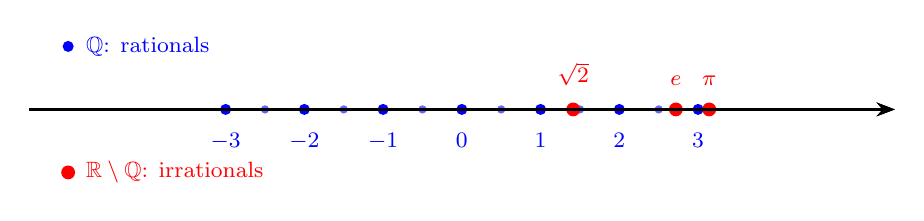
\begin{tikzpicture}[scale=1.0]
    % Number line
    \draw[-{Stealth},thick] (-5.5,0) -- (5.5,0);
    % Rational points
    \foreach \x/\lab in {-3/{-3}, -2/{-2}, -1/{-1}, 0/0, 1/1, 2/2, 3/3} {
      \fill[blue] (\x,0) circle (2pt);
      \node[blue, below=5pt] at (\x,0) {\footnotesize $\lab$};
    }
    % Some rationals between
    \foreach \x in {-2.5,-1.5,-0.5,0.5,1.5,2.5} {
      \fill[blue!60] (\x,0) circle (1.5pt);
    }
    % Irrational points (gaps filled)
    \fill[red] (1.414,0) circle (2.5pt);
    \node[red, above=5pt] at (1.414,0) {\footnotesize $\sqrt{2}$};
    \fill[red] (3.14159,0) circle (2.5pt);
    \node[red, above=5pt] at (3.14159,0) {\footnotesize $\pi$};
    \fill[red] (2.718,0) circle (2.5pt);
    \node[red, above=5pt] at (2.718,0) {\footnotesize $e$};
    % Legend
    \fill[blue] (-5.0,0.8) circle (2pt);
    \node[blue, right=3pt] at (-5.0,0.8) {\footnotesize $\mathbb{Q}$: rationals};
    \fill[red] (-5.0,-0.8) circle (2.5pt);
    \node[red, right=3pt] at (-5.0,-0.8) {\footnotesize $\mathbb{R} \setminus \mathbb{Q}$: irrationals};
    % Redraw number line on top
    \draw[-{Stealth},thick] (-5.5,0) -- (5.5,0);
  \end{tikzpicture}
  \end{center}

  \vspace{0.3em}
  $\mathbb{R}$ \alert{fills all the gaps} in $\mathbb{Q}$ --- it is a \emph{complete} ordered field.

  \note{
    This diagram shows the real number line. The blue dots represent rational
    numbers, which are scattered densely along the line but still leave gaps.
    The red dots represent irrationals like the square root of 2, e, and pi,
    which fill those gaps. The real numbers form a complete number line with
    no gaps at all. This is precisely what the least-upper-bound property
    guarantees. Now let's see what powerful consequences follow from this
    completeness.
  }
\end{frame}

% =============================================================================
% SECTION 2: THE ARCHIMEDEAN PROPERTY AND DENSITY OF Q
% =============================================================================

\section{Archimedean Property and Density of $\mathbb{Q}$}

% --- Theorem 1.20 statement: Build 1/2 ---
\begin{frame}{Theorem 1.20: Two Key Consequences}
  \begin{thmblock}{Theorem 1.20(a) --- Archimedean Property}
    If $x \in \mathbb{R}$, $y \in \mathbb{R}$, and $x > 0$, then there is a positive integer $n$ such that
    \[
      nx > y.
    \]
  \end{thmblock}

  \note{
    Our first major consequence of the least-upper-bound property is the
    archimedean property. It says: given any two positive real numbers x and y,
    no matter how small x is and how large y is, if you add x to itself enough
    times, you will eventually exceed y. In other words, there are no
    infinitely large or infinitely small real numbers.
  }
\end{frame}

% --- Theorem 1.20 statement: Build 2/2 ---
\begin{frame}{Theorem 1.20: Two Key Consequences}
  \begin{thmblock}{Theorem 1.20(a) --- Archimedean Property}
    If $x \in \mathbb{R}$, $y \in \mathbb{R}$, and $x > 0$, then there is a positive integer $n$ such that
    \[
      nx > y.
    \]
  \end{thmblock}

  \vspace{0.5em}
  \begin{thmblock}{Theorem 1.20(b) --- Density of $\mathbb{Q}$ in $\mathbb{R}$}
    If $x \in \mathbb{R}$, $y \in \mathbb{R}$, and $x < y$, then there exists $p \in \mathbb{Q}$ such that
    \[
      x < p < y.
    \]
  \end{thmblock}

  \note{
    The second consequence is the density of the rationals in the reals.
    Between any two distinct real numbers, no matter how close together, there
    is always a rational number. This means the rationals are, in a sense,
    spread everywhere throughout the real line. Let's look at a diagram to
    build some intuition.
  }
\end{frame}

% --- Terminology ---
\begin{frame}{Terminology}
  \begin{itemize}
    \item Part (a) is the \alert{archimedean property} of $\mathbb{R}$:

    \vspace{0.3em}
    No element of $\mathbb{R}$ is ``infinitely large'' relative to any other.

    \vspace{0.8em}
    \item Part (b) says $\mathbb{Q}$ is \alert{dense} in $\mathbb{R}$:

    \vspace{0.3em}
    Between any two reals, there is a rational.
  \end{itemize}

  \note{
    Let's clarify the terminology. The archimedean property means there are no
    infinitely large elements: you can always reach any real number by adding
    up enough copies of any positive real number. The density of Q in R means
    that no matter how close two real numbers are, you can always squeeze a
    rational number between them. Let's see visual illustrations of both
    properties, starting with the archimedean property.
  }
\end{frame}

% --- Diagram: Archimedean property ---
\begin{frame}{Archimedean Property: Illustration}
  \begin{center}
  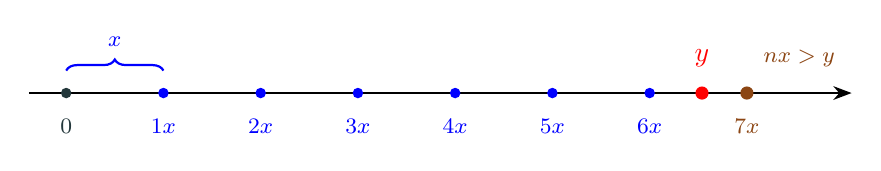
\begin{tikzpicture}[scale=0.95]
    % Number line
    \draw[-{Stealth},thick] (-0.5,0) -- (10.5,0);
    % Origin
    \fill[mDarkTeal] (0,0) circle (2pt) node[below=6pt] {\footnotesize $0$};
    % x marks
    \foreach \i in {1,2,3,4,5,6} {
      \fill[blue] (\i*1.3,0) circle (2pt);
      \node[blue, below=6pt] at (\i*1.3,0) {\footnotesize $\i x$};
    }
    % y mark
    \fill[red] (8.5,0) circle (2.5pt);
    \node[red, above=6pt] at (8.5,0) {$y$};
    % Braces for x
    \draw[decorate, decoration={brace, amplitude=4pt}, thick, blue]
      (0,0.3) -- (1.3,0.3) node[midway, above=5pt] {\footnotesize $x$};
    % Label showing nx > y
    \node[mAccent, above=6pt] at (9.8,0) {\footnotesize $nx > y$};
    % Final point
    \fill[mAccent] (9.1,0) circle (2.5pt);
    \node[mAccent, below=6pt] at (9.1,0) {\footnotesize $7x$};
  \end{tikzpicture}
  \end{center}

  \vspace{0.3em}
  No matter how small $x > 0$ is, repeated addition \alert{eventually surpasses} any $y$.

  \note{
    This diagram illustrates the archimedean property. We start with a small
    positive number x, shown by the blue bracket, and keep adding copies of x:
    one x, two x, three x, and so on. No matter how large y is, we will
    eventually surpass it. There is no positive real number so small that its
    multiples stay bounded. Now let's visualize the other key consequence:
    the density of the rationals.
  }
\end{frame}

% --- Diagram: Density of Q ---
\begin{frame}{Density of $\mathbb{Q}$ in $\mathbb{R}$: Illustration}
  \begin{center}
  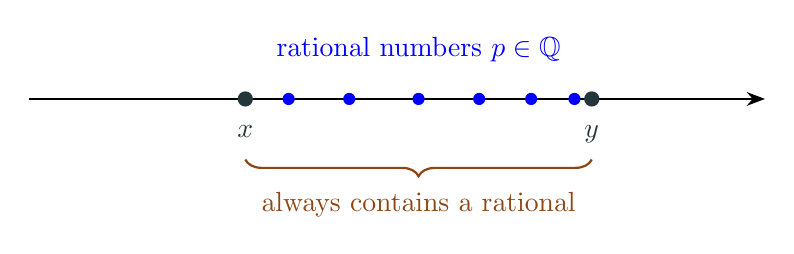
\begin{tikzpicture}[scale=1.1]
    % Number line
    \draw[-{Stealth},thick] (-0.5,0) -- (8,0);
    % x and y
    \fill[mDarkTeal] (2,0) circle (2.5pt) node[below=6pt] {$x$};
    \fill[mDarkTeal] (6,0) circle (2.5pt) node[below=6pt] {$y$};
    % (interval highlight removed)
    % Rational points between
    \fill[blue] (2.5,0) circle (2pt);
    \fill[blue] (3.2,0) circle (2pt);
    \fill[blue] (4.0,0) circle (2pt);
    \fill[blue] (4.7,0) circle (2pt);
    \fill[blue] (5.3,0) circle (2pt);
    \fill[blue] (5.8,0) circle (2pt);
    % Label
    \node[blue, above=10pt] at (4.0,0) {rational numbers $p \in \mathbb{Q}$};
    % Brace
    \draw[decorate, decoration={brace, amplitude=6pt, mirror}, thick, mAccent]
      (2,-0.7) -- (6,-0.7) node[midway, below=8pt] {always contains a rational};
  \end{tikzpicture}
  \end{center}

  \note{
    Here we see the real number line with two arbitrary points x and y. The
    orange bracket shows the interval between them. No matter how close x and y
    are to each other, there are always rational numbers between them, shown as
    the blue dots. In fact, there are infinitely many rationals between any two
    reals. This is a remarkable property. Now let's prove both parts of
    Theorem 1.20.
  }
\end{frame}

% --- Proof of 1.20(a): Strategy ---
\begin{frame}{Proof of 1.20(a): Strategy}
  \textbf{Goal:} Show that for $x > 0$, the set $\{nx : n \in \mathbb{Z}^+\}$ is \alert{unbounded above}.

  \vspace{1em}
  \textbf{Technique:} Proof by contradiction using the least-upper-bound property.

  \vspace{1em}
  \textbf{Idea:}
  \begin{enumerate}
    \item Suppose the set $A = \{nx\}$ is bounded above.
    \item Then $\alpha = \sup A$ exists (by Theorem 1.19).
    \item Show this leads to a contradiction.
  \end{enumerate}

  \note{
    Let's prove the archimedean property. Our strategy is proof by
    contradiction. We consider the set A of all positive integer multiples of
    x, and assume for contradiction that this set is bounded above. Since R has
    the least-upper-bound property, A would then have a supremum. We will show
    this supremum cannot actually be an upper bound, giving us our
    contradiction.
  }
\end{frame}

% --- Proof of 1.20(a): Step 1 ---
\begin{frame}{Proof of 1.20(a)}
  \begin{proofblock}{Step 1: Setup}
    Let $A = \{nx : n \in \mathbb{Z}^+\}$.

    \vspace{0.3em}
    Suppose for contradiction that $A$ is bounded above (i.e., $nx \leq y$ for all $n$).

    \vspace{0.3em}
    By Theorem 1.19, $\alpha = \sup A$ exists.
  \end{proofblock}

  \note{
    Let A be the set of all positive integer multiples of x. If the archimedean
    property fails, then y is an upper bound of A. Since A is nonempty and
    bounded above, the least-upper-bound property gives us alpha equals the
    supremum of A.
  }
\end{frame}

% --- Proof of 1.20(a): Step 2 ---
\begin{frame}{Proof of 1.20(a)}
  \begin{proofblock}{Step 1: Setup}
    Let $A = \{nx : n \in \mathbb{Z}^+\}$.
    Suppose $\alpha = \sup A$ exists.
  \end{proofblock}

  \begin{proofblock}{Step 2: The contradiction}
    Since $x > 0$, we have $\alpha - x < \alpha$.

    \vspace{0.3em}
    So $\alpha - x$ is \emph{not} an upper bound of $A$.

    \vspace{0.3em}
    Hence $\alpha - x < mx$ for some positive integer $m$.

    \vspace{0.3em}
    But then $\alpha < (m+1)x \in A$. \alert{Contradiction!}
  \end{proofblock}

  \note{
    Here is the key step. Since x is positive, alpha minus x is strictly less
    than alpha. Since alpha is the least upper bound, alpha minus x cannot be
    an upper bound of A. Therefore, there exists some positive integer m such
    that m times x exceeds alpha minus x. But then m plus 1 times x exceeds
    alpha. Since m plus 1 times x is an element of A, we have found an element
    of A that exceeds alpha. This contradicts alpha being an upper bound of A.
    The archimedean property is proved. Now let's use it to prove the
    density of the rationals.
  }
\end{frame}

% --- Proof of 1.20(b): Strategy ---
\begin{frame}{Proof of 1.20(b): Strategy}
  \textbf{Goal:} Given $x < y$, find a rational $p = m/n$ with $x < m/n < y$.

  \vspace{1em}
  \textbf{Idea:} Use the archimedean property \emph{twice}:
  \begin{enumerate}
    \item Find $n$ large enough so that $1/n$ is smaller than $y - x$.
    \item Find the right integer $m$ so that $m/n$ lands between $x$ and $y$.
  \end{enumerate}

  \note{
    Now let's prove part b, the density of the rationals. We need to find a
    rational number m over n between x and y. The strategy uses the archimedean
    property twice. First, we use it to find an integer n large enough that 1
    over n is smaller than the gap y minus x. Then we use it again to find the
    right numerator m. Let's see the details.
  }
\end{frame}

% --- Proof of 1.20(b): Step 1 ---
\begin{frame}{Proof of 1.20(b)}
  \begin{proofblock}{Step 1: Make the mesh fine enough}
    Since $y - x > 0$, by part (a) there exists a positive integer $n$ with
    \[
      n(y - x) > 1.
    \]
  \end{proofblock}

  \note{
    Since y minus x is positive, we apply the archimedean property with x
    replaced by y minus x and y replaced by 1. This gives us a positive integer
    n such that n times the quantity y minus x exceeds 1. Equivalently, the
    spacing 1 over n is smaller than y minus x. This ensures our rational grid
    is fine enough to land a point inside the interval.
  }
\end{frame}

% --- Proof of 1.20(b): Step 2 ---
\begin{frame}{Proof of 1.20(b)}
  \begin{proofblock}{Step 1: Make the mesh fine enough}
    Find $n \in \mathbb{Z}^+$ with $n(y - x) > 1$.
  \end{proofblock}

  \begin{proofblock}{Step 2: Bound $nx$ between integers}
    By part (a), there exist positive integers $m_1, m_2$ with:
    \[
      m_1 > nx \quad \text{and} \quad m_2 > -nx.
    \]
    Hence $-m_2 < nx < m_1$, so there is an integer $m$ with
    \[
      m - 1 \leq nx < m.
    \]
  \end{proofblock}

  \note{
    Next, we apply the archimedean property again to find positive integers m 1
    and m 2 such that m 1 exceeds n times x and m 2 exceeds negative n times x.
    This means n times x is trapped between negative m 2 and m 1, so there must
    be an integer m that is the smallest integer exceeding n times x. In other
    words, m minus 1 is at most n times x, and n times x is strictly less
    than m.
  }
\end{frame}

% --- Proof of 1.20(b): Step 3 ---
\begin{frame}{Proof of 1.20(b)}
  \begin{proofblock}{Step 3: Combine the inequalities}
    From $nx < m$ and $n(y-x) > 1$:
    \[
      nx < m \leq 1 + nx < ny.
    \]
    Since $n > 0$:
    \[
      \boxed{x < \frac{m}{n} < y}
    \]
    Set $p = m/n \in \mathbb{Q}$. \qed
  \end{proofblock}

  \note{
    Now we combine everything. We know n times x is less than m, and m is at
    most 1 plus n times x. But 1 plus n times x is less than n times y, since n
    times the quantity y minus x exceeds 1. Dividing through by the positive
    integer n, we get x is less than m over n, which is less than y. So p equals
    m over n is the rational number we were looking for. The density of Q in R
    is proved. Let's see a visual summary of this proof idea.
  }
\end{frame}

% --- Diagram: Proof idea for 1.20(b) ---
\begin{frame}{Proof of 1.20(b): Visual Summary}
  \begin{center}
  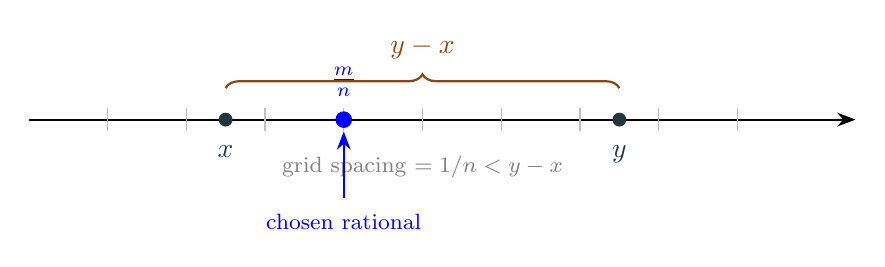
\begin{tikzpicture}[scale=1.0]
    % Number line
    \draw[-{Stealth},thick] (-0.5,0) -- (10,0);
    % x and y
    \fill[mDarkTeal] (2,0) circle (2.5pt) node[below=6pt] {$x$};
    \fill[mDarkTeal] (7,0) circle (2.5pt) node[below=6pt] {$y$};
    % Gap
    \draw[decorate, decoration={brace, amplitude=5pt}, thick, mAccent]
      (2,0.4) -- (7,0.4) node[midway, above=7pt] {$y - x$};
    % Grid points at spacing 1/n
    \foreach \x in {0.5,1.5,2.5,3.5,4.5,5.5,6.5,7.5,8.5} {
      \draw[gray!50] (\x,-0.15) -- (\x,0.15);
    }
    \node[gray] at (4.5,-0.6) {\footnotesize grid spacing $= 1/n < y - x$};
    % The chosen m/n
    \fill[blue] (3.5,0) circle (3pt);
    \node[blue, above=5pt] at (3.5,0) {$\frac{m}{n}$};
    % Arrow
    \draw[-{Stealth}, blue, thick] (3.5,-1.0) -- (3.5,-0.15);
    \node[blue] at (3.5,-1.3) {\footnotesize chosen rational};
  \end{tikzpicture}
  \end{center}

  \note{
    This diagram summarizes the proof idea. The key insight is to choose a
    denominator n large enough that the grid spacing 1 over n is smaller than
    the gap y minus x. Once the grid is that fine, at least one grid point m
    over n must fall inside the interval from x to y. It's a beautifully simple
    argument once you have the archimedean property. Next, we turn to another
    important consequence of the least-upper-bound property: the existence of
    nth roots.
  }
\end{frame}

% =============================================================================
% SECTION 3: EXISTENCE OF NTH ROOTS
% =============================================================================

\section{Existence of $n$th Roots}

% --- Theorem 1.21 statement ---
\begin{frame}{Theorem 1.21: Existence of $n$th Roots}
  \begin{thmblock}{Theorem 1.21}
    For every real $x > 0$ and every integer $n > 0$, there is \alert{one and only one} positive real $y$ such that
    \[
      y^n = x.
    \]
  \end{thmblock}

  \vspace{0.5em}
  This number $y$ is written $\sqrt[n]{x}$ or $x^{1/n}$.

  \note{
    Now we come to a beautiful application of the least-upper-bound property.
    Theorem 1.21 says that every positive real number has a unique positive nth
    root. This directly resolves the problem from the introduction: while the
    square root of 2 does not exist in the rationals, it does exist in the
    reals. The proof will show exactly how the least-upper-bound property fills
    the gap.
  }
\end{frame}

% --- Proof Strategy ---
\begin{frame}{Proof Strategy: Theorem 1.21}
  \textbf{Goal:} Find $y > 0$ with $y^n = x$.

  \vspace{0.8em}
  \textbf{Approach:}
  \begin{enumerate}
    \item \textbf{Uniqueness:} If $0 < y_1 < y_2$, then $y_1^n < y_2^n$. At most one root.
    \item \textbf{Define} $E = \{t > 0 : t^n < x\}$.
    \item \textbf{Show} $E \neq \emptyset$ and $E$ is bounded above. Set $y = \sup E$.
    \item \textbf{Rule out} $y^n < x$: build $h > 0$ with $(y+h)^n < x$, so $y+h \in E$ --- contradicts $y$ being an \alert{upper bound}.
    \item \textbf{Rule out} $y^n > x$: build $k > 0$ with $(y-k)^n > x$, so $y-k$ is an upper bound --- contradicts $y$ being the \alert{least} upper bound.
  \end{enumerate}

  \note{
    Here is the proof strategy. Uniqueness is immediate: the function t to the
    n is strictly increasing on positive reals. For existence, we define E to
    be the set of all positive reals t whose nth power is less than x. We take
    y to be the supremum of E, which exists by the least-upper-bound property.
    Then we prove y to the n equals x by ruling out both alternatives. If y to
    the n were less than x, we would construct a small positive number h so
    that y plus h is still in E, contradicting the fact that y is an upper
    bound of E. If y to the n were greater than x, we would construct a small
    positive k so that y minus k is already an upper bound of E, contradicting
    the fact that y is the least upper bound.
  }
\end{frame}

% --- Proof Step 1: Uniqueness ---
\begin{frame}{Proof of Theorem 1.21 --- Step 1: Uniqueness}
  \begin{proofblock}{Step 1: At most one such $y$}
    If $0 < y_1 < y_2$, then
    \[
      y_1^n < y_2^n.
    \]
    So there is \alert{at most one} positive real $y$ with $y^n = x$.
  \end{proofblock}

  \note{
    The uniqueness part is straightforward. If y 1 is less than y 2, and both
    are positive, then y 1 to the n is strictly less than y 2 to the n. This
    follows because multiplication by a positive number preserves inequalities.
    Therefore, the equation y to the n equals x can have at most one positive
    solution. Now we need to show that at least one such y exists.
  }
\end{frame}

% --- Proof Step 2: Define E ---
\begin{frame}{Proof of Theorem 1.21 --- Step 2: Define $E$}
  \begin{proofblock}{Step 2: Define the set $E$}
    Let
    \[
      E = \{t \in \mathbb{R} : t > 0 \text{ and } t^n < x\}.
    \]
  \end{proofblock}

  \vspace{0.5em}
  \textbf{$E$ is not empty:} Take $t = \dfrac{x}{1+x}$. Then $0 < t < 1$, so $t^n \leq t < x$.

  \vspace{0.5em}
  \textbf{$E$ is bounded above:} If $t > 1 + x$, then $t^n \geq t > x$, so $t \notin E$.

  \note{
    We define E to be the set of all positive reals t whose nth power is less
    than x. We need to check E is nonempty and bounded above. For nonempty:
    take t equals x over 1 plus x. This number lies strictly between 0 and 1,
    and raising a number in that range to a positive power only makes it
    smaller, so t to the n is at most t, which is less than x. So t belongs
    to E. For bounded above: if t exceeds 1 plus x, then since t is greater
    than 1, t to the n is at least t, which exceeds x. So 1 plus x is an
    upper bound of E.
  }
\end{frame}

% --- Proof Step 3: y = sup E ---
\begin{frame}{Proof of Theorem 1.21 --- Step 3: $y = \sup E$}
  \begin{proofblock}{Step 3: Apply Theorem 1.19}
    Since $E \neq \emptyset$ and $E$ is bounded above, Theorem 1.19 gives:
    \[
      y = \sup E.
    \]
  \end{proofblock}

  \vspace{0.5em}
  \textbf{Claim:} $y^n = x$.

  \note{
    By the least-upper-bound property, the supremum y of E exists. Our claim is
    that y to the n equals x. As outlined in the strategy, we will establish
    this by ruling out the two alternatives: y to the n less than x, and y to
    the n greater than x. Before handling them, we pause to record the key
    algebraic inequality that both cases will need.
  }
\end{frame}

% --- Proof Step 4: Key inequality ---
\begin{frame}{Proof of Theorem 1.21 --- Key Inequality}
  \begin{proofblock}{Key algebraic identity}
    For $0 < a < b$:
    \[
      b^n - a^n = (b - a)\bigl(b^{n-1} + b^{n-2}a + \cdots + a^{n-1}\bigr)
    \]
    The second factor has $n$ terms, each $\leq b^{n-1}$, so:
    \[
      \boxed{b^n - a^n < (b - a)\,n\,b^{n-1}}
    \]
  \end{proofblock}

  \note{
    Before we handle the two cases, we need a key algebraic inequality. The
    factorization of b to the n minus a to the n gives us b minus a times a sum
    of n terms. When a is less than b, each term in that sum is at most b to
    the n minus 1. So the entire sum is at most n times b to the n minus 1.
    This gives us the boxed upper bound, which we will use in both cases of
    the proof.
  }
\end{frame}

% --- Proof Step 5: Case y^n < x ---
\begin{frame}{Proof of Theorem 1.21 --- Case: $y^n < x$}
  \begin{proofblock}{Case 1: Suppose $y^n < x$ --- derive contradiction}
    Choose $h$ with $0 < h < 1$ and
    \[
      h < \frac{x - y^n}{n(y+1)^{n-1}}.
    \]
    Set $a = y$, $b = y + h$. Then:
    \[
      (y+h)^n - y^n < h\,n\,(y+h)^{n-1} < h\,n\,(y+1)^{n-1} < x - y^n.
    \]
    So $(y+h)^n < x$, meaning $y + h \in E$.

    \vspace{0.3em}
    But $y + h > y = \sup E$. \alert{Contradiction!}
  \end{proofblock}

  \note{
    Assume y to the n is less than x. We choose a small positive h, less than
    1, and small enough that h times n times the quantity y plus 1 to the n
    minus 1 is less than x minus y to the n. Applying our key inequality, the
    chain of inequalities on the slide shows that y plus h to the n is still
    less than x. So y plus h belongs to E, but y plus h exceeds y. This
    contradicts y being an upper bound of E. Now let's handle the other case.
  }
\end{frame}

% --- Proof Step 6: Case y^n > x ---
\begin{frame}{Proof of Theorem 1.21 --- Case: $y^n > x$}
  \begin{proofblock}{Case 2: Suppose $y^n > x$ --- derive contradiction}
    Put
    \[
      k = \frac{y^n - x}{n\,y^{n-1}}.
    \]
    Then $0 < k < y$. By the key inequality (with $a = y-k$, $b = y$):
    \[
      y^n - (y-k)^n < k\,n\,y^{n-1} = y^n - x,
    \]
    so $(y-k)^n > x$. Hence $y - k$ is an \alert{upper bound} of $E$.

    \vspace{0.3em}
    But $y - k < y = \sup E$. \alert{Contradiction!}
  \end{proofblock}

  \note{
    Now assume y to the n is greater than x. We define k as shown, which is
    positive and less than y. Applying the key inequality with a equal to y
    minus k and b equal to y, we find that y to the n minus the quantity y
    minus k to the n is strictly less than y to the n minus x. So y minus k
    to the n is greater than x, which means y minus k is an upper bound of E.
    But y minus k is strictly less than y, contradicting that y is the least
    upper bound. Both cases lead to contradictions, so y to the n must equal
    x. The proof is complete.
  }
\end{frame}

% --- Diagram: Proof of 1.21 ---
\begin{frame}{Proof of Theorem 1.21: Visual Summary}
  \begin{center}
  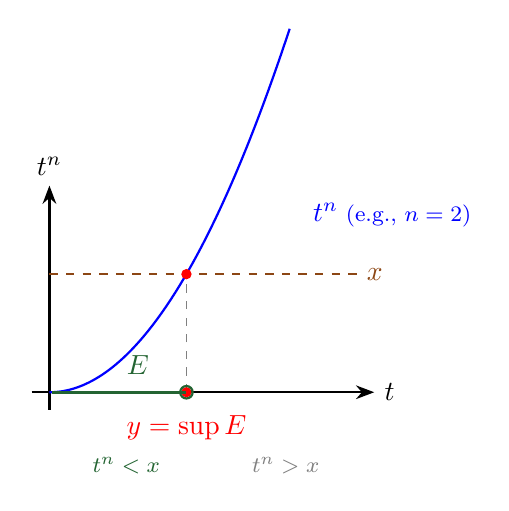
\begin{tikzpicture}[scale=0.75]
    % Axes
    \draw[-{Stealth},thick] (-0.3,0) -- (5.5,0) node[right] {$t$};
    \draw[-{Stealth},thick] (0,-0.3) -- (0,3.5) node[above] {$t^n$};
    % Curve t^n (shorter range so it stays within axes)
    \draw[thick, blue, domain=0:1.85, samples=80] plot (\x*2.2, {(\x)^2 * 1.8});
    \node[blue, right] at (4.3,3.0) {$t^n$\;\footnotesize(e.g., $n=2$)};
    % Horizontal line at x
    \draw[dashed, mAccent, thick] (0,2.0) -- (5.2,2.0) node[right] {$x$};
    % y = sup E
    \draw[dashed, gray] (2.32,0) -- (2.32,2.0);
    \fill[red] (2.32,0) circle (2.5pt) node[below=5pt] {$y = \sup E$};
    \fill[red] (2.32,2.0) circle (2.5pt);
    % E region (open interval: does not include y)
    \draw[very thick, proofcolor] (0.05,0) -- (2.32,0);
    \draw[proofcolor, thick] (2.32,0) circle (3pt);
    \node[proofcolor, above=3pt] at (1.5,0) {$E$};
    % Labels
    \node[proofcolor, below=20pt] at (1.3,0) {\footnotesize $t^n < x$};
    \node[gray, below=20pt] at (4.0,0) {\footnotesize $t^n > x$};
  \end{tikzpicture}
  \end{center}

  \note{
    This diagram shows the function t to the n as the blue curve. The
    horizontal dashed line is at height x. The set E, shown in green, consists
    of all positive t where the curve lies below x. The supremum y is where the
    curve meets the line. If y to the n were less than x, we could move right
    and stay in E. If y to the n were greater than x, we could find a smaller
    upper bound by moving left. So y to the n must equal x exactly. Now let's
    look at a nice corollary of this result.
  }
\end{frame}

% =============================================================================
% SECTION 4: COROLLARY AND DECIMALS
% =============================================================================

\section{Corollary and Decimal Expansions}

% --- Corollary to 1.21 ---
\begin{frame}{Corollary to Theorem 1.21}
  \begin{thmblock}{Corollary}
    If $a, b > 0$ are real and $n$ is a positive integer, then
    \[
      \boxed{(ab)^{1/n} = a^{1/n}\, b^{1/n}.}
    \]
  \end{thmblock}

  \note{
    A nice consequence of the uniqueness part of Theorem 1.21 is this corollary
    about nth roots of products. The nth root of a product equals the product
    of the nth roots. This is a familiar rule, but it requires the existence
    and uniqueness of nth roots to make rigorous. Let's see the short proof.
  }
\end{frame}

% --- Proof of Corollary ---
\begin{frame}{Proof of the Corollary}
  \begin{proofblock}{Proof}
    Put $\alpha = a^{1/n}$ and $\beta = b^{1/n}$. Then:
    \[
      ab = \alpha^n \beta^n = (\alpha\beta)^n
    \]
    by commutativity of multiplication (Axiom M2, Definition 1.12).

    \vspace{0.5em}
    By the \alert{uniqueness} in Theorem 1.21:
    \[
      (ab)^{1/n} = \alpha\beta = a^{1/n}\, b^{1/n}. \quad \qed
    \]
  \end{proofblock}

  \note{
    The proof is elegant and short. Let alpha be the nth root of a and beta be
    the nth root of b. Then a times b equals alpha to the n times beta to the
    n, which equals alpha beta to the n, by commutativity of multiplication.
    Now, alpha beta is a positive real number whose nth power equals a b. By
    the uniqueness assertion of Theorem 1.21, it must be the nth root of a b.
    That completes the proof. We finish the section with a brief look at
    decimal expansions.
  }
\end{frame}

% --- 1.22 Decimals: Build 1/2 ---
\begin{frame}{1.22: Decimals}
  Let $x > 0$ be real. Define a sequence of digits:

  \vspace{0.5em}
  \begin{itemize}
    \item $n_0$ = largest integer $\leq x$ \quad {\footnotesize (exists by archimedean property)}
    \item $n_k$ = largest integer such that
    \begin{equation}
      n_0 + \frac{n_1}{10} + \cdots + \frac{n_k}{10^k} \leq x \tag{5}
    \end{equation}
  \end{itemize}

  \note{
    We conclude this section with a brief discussion of decimal expansions.
    Given a positive real number x, we can construct its decimal expansion as
    follows. First, let n 0 be the largest integer that does not exceed x. This
    exists by the archimedean property. Then, having chosen the digits n 0
    through n k minus 1, let n k be the largest integer such that the partial
    decimal sum does not exceed x.
  }
\end{frame}

% --- 1.22 Decimals: Build 2/2 ---
\begin{frame}{1.22: Decimals}
  Let $x > 0$ be real. Define a sequence of digits:

  \vspace{0.5em}
  \begin{itemize}
    \item $n_0$ = largest integer $\leq x$ \quad {\footnotesize (exists by archimedean property)}
    \item $n_k$ = largest integer such that
    \begin{equation}
      n_0 + \frac{n_1}{10} + \cdots + \frac{n_k}{10^k} \leq x \tag{5}
    \end{equation}
  \end{itemize}

  \vspace{0.3em}
  Let $E$ be the set of all such partial sums. Then $x = \sup E$.

  \vspace{0.3em}
  The \alert{decimal expansion} of $x$ is:
  \begin{equation}
    n_0 \cdot n_1 n_2 n_3 \cdots \tag{6}
  \end{equation}

  \note{
    The set E of all these partial decimal sums is bounded above by x itself.
    The crucial fact is that x equals the supremum of E. This connects the
    decimal representation to the least-upper-bound property. Conversely, any
    infinite decimal defines a bounded set of partial sums, whose supremum is
    the real number it represents. Since we will not use decimals in the rest
    of the book, we do not pursue this further. Let's wrap up with a summary
    of the key results from this section.
  }
\end{frame}

% =============================================================================
% SUMMARY
% =============================================================================

\section{Summary}

% --- Summary: Build 1/4 ---
\begin{frame}{Summary}
  \textbf{Key takeaways from this section:}
  \begin{itemize}
    \item \textbf{Theorem 1.19:} $\mathbb{R}$ exists as an ordered field with the least-upper-bound property, containing $\mathbb{Q}$
  \end{itemize}

  \note{
    Let's summarize what we covered in this section. The foundational result is
    Theorem 1.19: the real numbers exist as an ordered field with the
    least-upper-bound property, and they contain the rationals as a subfield.
    Everything else in this section flows from this single powerful property.
  }
\end{frame}

% --- Summary: Build 2/4 ---
\begin{frame}{Summary}
  \textbf{Key takeaways from this section:}
  \begin{itemize}
    \item \textbf{Theorem 1.19:} $\mathbb{R}$ exists as an ordered field with the least-upper-bound property, containing $\mathbb{Q}$
    \item \textbf{Theorem 1.20(a):} Archimedean property --- no infinitely large elements
  \end{itemize}

  \note{
    The archimedean property, Theorem 1.20 part a, tells us that the reals
    have no infinitely large or infinitely small elements relative to one
    another. You can always exceed any real number by adding up enough copies
    of any positive real number, no matter how small.
  }
\end{frame}

% --- Summary: Build 3/4 ---
\begin{frame}{Summary}
  \textbf{Key takeaways from this section:}
  \begin{itemize}
    \item \textbf{Theorem 1.19:} $\mathbb{R}$ exists as an ordered field with the least-upper-bound property, containing $\mathbb{Q}$
    \item \textbf{Theorem 1.20(a):} Archimedean property --- no infinitely large elements
    \item \textbf{Theorem 1.20(b):} $\mathbb{Q}$ is dense in $\mathbb{R}$ --- rationals are everywhere
  \end{itemize}

  \note{
    Part b of Theorem 1.20 shows that the rationals are dense in the reals:
    between any two real numbers, no matter how close together, you can always
    find a rational number sitting between them. We proved this using the
    archimedean property to make the rational grid fine enough to land a point
    inside any interval.
  }
\end{frame}

% --- Summary: Build 4/4 ---
\begin{frame}{Summary}
  \textbf{Key takeaways from this section:}
  \begin{itemize}
    \item \textbf{Theorem 1.19:} $\mathbb{R}$ exists as an ordered field with the least-upper-bound property, containing $\mathbb{Q}$
    \item \textbf{Theorem 1.20(a):} Archimedean property --- no infinitely large elements
    \item \textbf{Theorem 1.20(b):} $\mathbb{Q}$ is dense in $\mathbb{R}$ --- rationals are everywhere
    \item \textbf{Theorem 1.21:} Every positive real has a unique $n$th root
  \end{itemize}

  \vspace{0.8em}
  \textbf{Coming up next:} The extended real number system ($+\infty$ and $-\infty$).

  \note{
    Finally, Theorem 1.21 establishes that every positive real number has a
    unique nth root. This resolves the problem of the square root of 2 that
    motivated the entire chapter. All three results flow from the single
    powerful assumption that R has the least-upper-bound property. In the next
    section, we will extend the real number system by adding positive infinity
    and negative infinity, creating the extended real number system.
  }
\end{frame}

\end{document}
